%%% Richard James Howe 2/2
%% Final Year Project poster presentation.
% This uses a package called 'baposter.cls' which can be
% found here: http://www.brian-amberg.de/uni/poster/
% This package has been written by Brian Amberg (baposter@brian-amberg.de)

\documentclass[a1paper,portrait]{baposter}

\usepackage{relsize}    % For \smaller
\usepackage{url}      % For \url
\usepackage{epstopdf}  % Included EPS files automatically converted to PDF to include with pdflatex

%%% Global Settings %%%%%%%%%%%%%%%%%%%%%%%%%%%%%%%%%%%%%%%%%%%%%%%%%%%%%%%%%%%

\graphicspath{{pix/}}  % Root directory of the pictures 
\tracingstats=2      % Enabled LaTeX logging with conditionals

%%% Color Definitions %%%%%%%%%%%%%%%%%%%%%%%%%%%%%%%%%%%%%%%%%%%%%%%%%%%%%%%%%

\definecolor{bordercol}{RGB}{40,40,40}
\definecolor{headercol1}{RGB}{186,215,230}
\definecolor{headercol2}{RGB}{80,80,80}
\definecolor{headerfontcol}{RGB}{0,0,0}
\definecolor{boxcolor}{RGB}{186,215,230}

%%%%%%%%%%%%%%%%%%%%%%%%%%%%%%%%%%%%%%%%%%%%%%%%%%%%%%%%%%%%%%%%%%%%%%%%%%%%%%%%
%%% Utility functions %%%%%%%%%%%%%%%%%%%%%%%%%%%%%%%%%%%%%%%%%%%%%%%%%%%%%%%%%%

%%% Save space in lists. Use this after the opening of the list %%%%%%%%%%%%%%%%
\newcommand{\compresslist}{
  \setlength{\itemsep}{1pt}
  \setlength{\parskip}{0pt}
  \setlength{\parsep}{0pt}
}

%%%%%%%%%%%%%%%%%%%%%%%%%%%%%%%%%%%%%%%%%%%%%%%%%%%%%%%%%%%%%%%%%%%%%%%%%%%%%%%
%%% Document Start %%%%%%%%%%%%%%%%%%%%%%%%%%%%%%%%%%%%%%%%%%%%%%%%%%%%%%%%%%%%
%%%%%%%%%%%%%%%%%%%%%%%%%%%%%%%%%%%%%%%%%%%%%%%%%%%%%%%%%%%%%%%%%%%%%%%%%%%%%%%

\begin{document}
\typeout{Poster rendering started}

%%% Setting Background Image %%%%%%%%%%%%%%%%%%%%%%%%%%%%%%%%%%%%%%%%%%%%%%%%%%
\background{
  \begin{tikzpicture}[remember picture,overlay]%
  \draw (current page.north west)+(-2em,2em) node[anchor=north west]
  {
\includegraphics[height=1.1\textheight]{background}};
  \end{tikzpicture}
}

\begin{poster}{
  grid=false,
  borderColor=bordercol,
  headerColorOne=headercol1,
  headerColorTwo=headercol2,
  headerFontColor=headerfontcol,
  boxColorOne=boxcolor,
  headershape=roundedright,
  headerfont=\large\sf\bf,
  textborder=rectangle,
  background=user,
  headerborder=open,
  boxshade=plain
}
{
  Eye Catcher, empty if option eyecatcher=false - unused
}
{\Large\sf\bf
  A VHDL based educational computer (2/2).
}
{
  \vspace{1em} Richard James Howe : 082060589\\
  {\smaller howe.r.j.89@gmail.com}
}
{
\setlength\fboxsep{0pt}
\setlength\fboxrule{0.5pt}
  \fbox{
    \begin{minipage}{10em}
      
\includegraphics[width=10em,height=4em]{aston.jpg}
    \end{minipage}
  }
}

\headerbox{Problems Faced}{name=problemsfaced,column=0,row=0}{
\scriptsize
The main problems I faced were; slow development time due to the time it
takes to synthesize code, there is no way apart from using faster computers
to reduce this time, however the addition of a bootloader means that
you no longer have to keep synthesizing code. Secondly there was the problem
of developing adequate methods for testing the toolchain, if there is a
bug it could be in one of the following; The build process, the FORTH
interpreter, the assembler, the VHDL simulation or the actual hardware
implementation of the VHDL.
}

\headerbox{Future plans}{name=futureplans,column=0,below=problemsfaced, above=bottom}{
\smaller                          % Make the whole text smaller
I plan on continuing the project beyond the original scope, there is still plenty
of room on the device and would like to add units that are useful to me and fellow
engineers, more specifically engineering students.

These modules would include signal generators, Ethernet interface, on board memory
interfaces, data loggers and much more. I would also like to continue on and expand
the firmware on board to create a more standalone system. Some of these would however
mean the creation of external plug-in boards as well. One peripheral which the
FPGA is quite suited to would be the addition of a logic analyser, this would not
be too difficult to add and would be of great benefit. Of great use would be a
USB keyboard to act as input as well.

I did add a multiplier to the instruction set, however it delayed the logic too
much which would have reduced the overall speed of the CPU, adding the multiplier
back in as a peripheral or optimizing the CPU would both be options.

In summary:
\begin{itemize}
  \item Optimize CPU.
  \item Improve firmware, including a full blown interpreter.
  \item Add analogue interface peripherals and electronics.
  \item Either add multiplier to optimized CPU or add multiplier
  as a two clock cycle to execute peripheral.
\end{itemize}
} 

\headerbox{How it works}{name=howitworks,span=2,column=1,row=0}{
\scriptsize
\subsection{CPU Core}
The diagram bellow shows how data moves through the H2 (The name of this
CPU), the processor can execute one instruction per clock cycle and has room for
further customization.

\begin{center}
    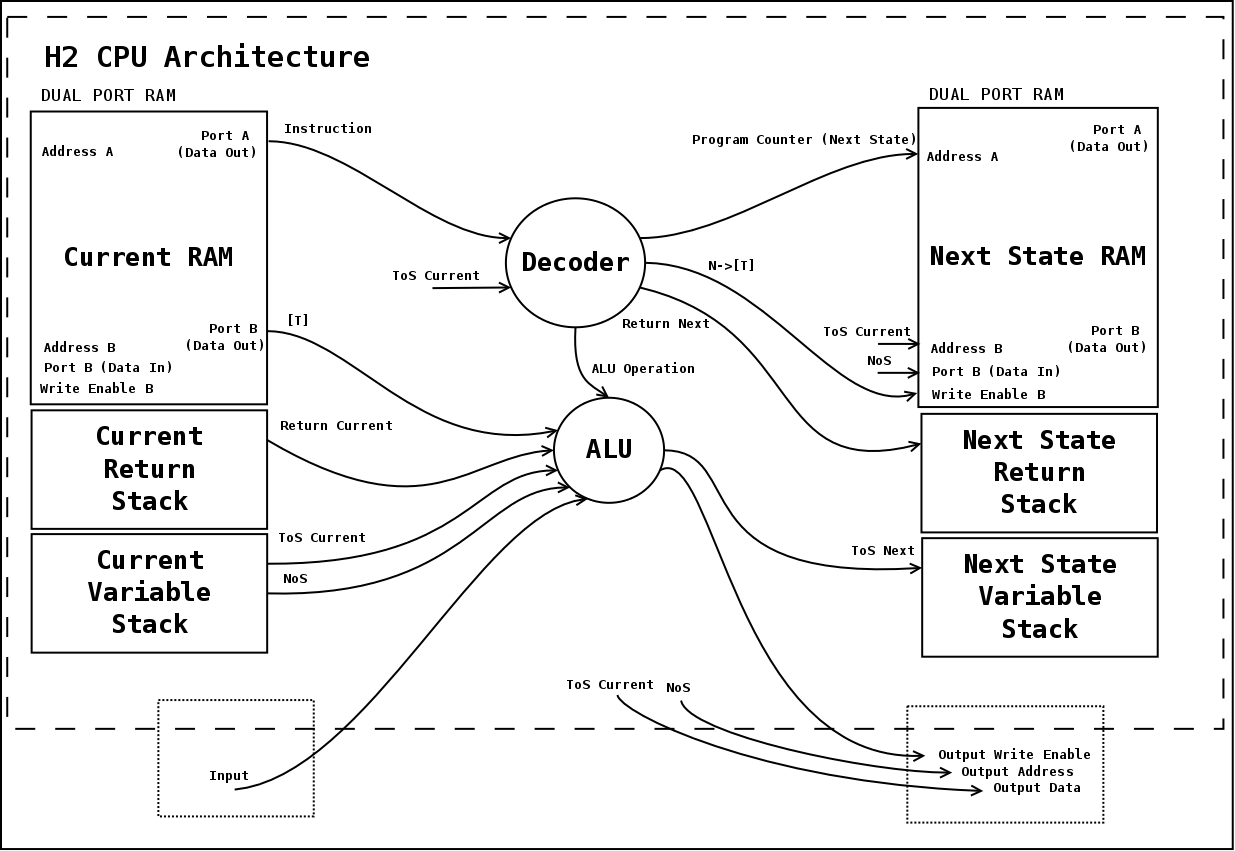
\includegraphics[scale=0.12]{h2.png}
\end{center}

For a detailed view consult the code hosted on Github.

\subsection{VGA Test Pattern}
\begin{center}
    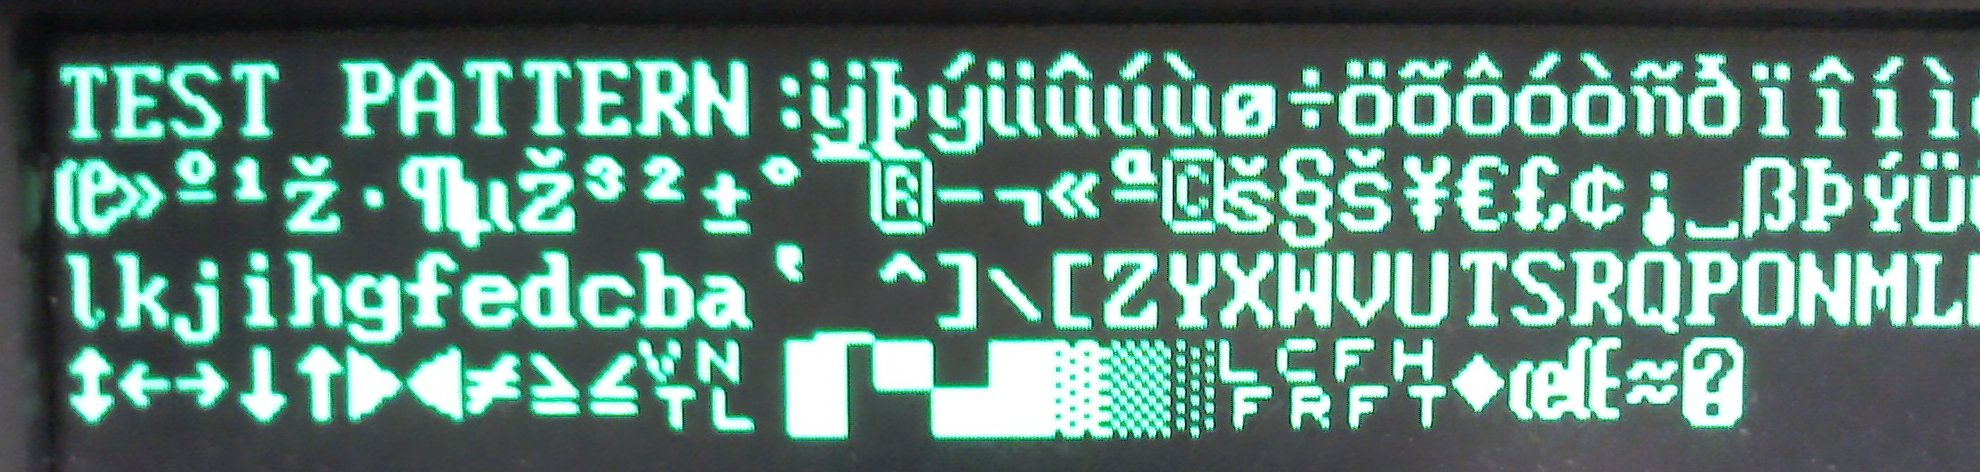
\includegraphics[scale=0.1]{testVGA.jpg}
\end{center}

You can see here the test pattern from the VGA output[2], this can be changed
given the right software running. It is controlled by the CPU via a block of
shared dual port RAM.

\subsection{UART and other}

Also included is a UART[3] that can be used either as a human interface or to transfer
data to and from the device. The other peripherals included use the devices switches,
buttons and LEDs to provide simpler and more obvious input.
}
\headerbox{Design Goals}
{name=firmware,span=2,column=1,below=howitworks,above=bottom}{
\scriptsize
\subsection{Extensibility}
Both the CPU core and the system itself are extensible, you can modify both. The CPU by adding
more instructions, the system as a whole by adding new devices to the interface list. I have
added VGA support by including a VGA core available on \url{opencores.org}[4].
\subsection{Modularity and Code reuse}
I want to be able to reuse the code I have written for this project in future projects, and
this is possible due to the way the project has been designed, from the FORTH interpreter
written in C to each of the cores, they can easily be reused.
\subsection{Small}
One of the goals of this project was to create a \emph{small} system so it could sit
comfortably alongside other designs while still providing a customizable System On (a)
Chip (SoC).
}

\end{poster}
\end{document}
